\documentclass[a4paper,12pt,twoside]{scrreprt}
% Autor der Vorlage: Klaus Rheinberger, FH Vorarlberg
% 2017-02-20

%% Hilfe: z.B.
% empfohlener Einstieg: http://latex.tugraz.at/
% https://de.wikibooks.org/wiki/LaTeX-Kompendium:_Schnellkurs:_Erste_Schritte
% https://de.wikibooks.org/wiki/LaTeX-Kompendium:_Schnellkurs
% https://de.wikibooks.org/wiki/LaTeX-Kompendium

%% Pakete:
% Der Befehl \usepackage[latin9]{inputenc} ermöglicht die direkte Angabe von Umlauten. Übrigens lässt sich so auch das Euro-Zeichen direkt eingeben. Auf Betriebssystemen, wie zum Beispiel allen neueren Linux-Distributionen, verwendet man statt \usepackage[latin9]{inputenc} besser \usepackage[utf8]{inputenc}, auf Applesystemen verwendet man \usepackage[macce]{inputenc} (oder das für ältere Modelle gültige \usepackage[applemac]{inputenc}).
\usepackage[utf8]{inputenc}
\usepackage[T1]{fontenc}    % Silbentrennung bei Sonderzeichen
\usepackage{graphicx}	    % Bilder einbinden
\usepackage[english]{babel} % Deutsche Sprachanpassungen
\usepackage{csquotes}	    % When using babel or polyglossia with biblatex, loading csquotes is recommended to ensure that quoted texts are typeset according to the rules of your main language.
\usepackage{acronym}  % für optionales Abkürzungsverzeichnis
\usepackage{eurosym}  % z. B. \EUR{12345,68}
\usepackage[linktocpage=true]{hyperref} % Links z. B. \href{https://www.wikibooks.org}{Wikibooks home}
\usepackage[bindingoffset=8mm]{geometry}% Bindeverlust von 8mm einbeziehen. Mit dem geometry-Paket können Sie die Ränder auch ganz individuell anpassen.
\usepackage{caption} % Abbildungslegenden
\captionsetup{format=hang, justification=raggedright}
\usepackage{placeins}
\usepackage{float} % prevent LaTeX table repositioning

% sql formatting
\usepackage{listings}
\usepackage{xcolor}
\lstdefinestyle{sql}{
  language=SQL,
  basicstyle=\ttfamily\small,
  keywordstyle=\color{blue}\bfseries,
  commentstyle=\color{gray},
  stringstyle=\color{orange},
  morekeywords={SELECT, FROM, WHERE, JOIN, AND, OR, EXISTS, BETWEEN, AS, ON,
      HAVING},
  breaklines=true,
  frame=single,
  captionpos=b
}

\usepackage[a-2b,mathxmp]{pdfx}[2018/12/22]

\usepackage[style=ieee,citestyle=ieee,backend=biber]{biblatex}
% Literaturverweise
%\usepackage[style=numeric,citestyle=numeric,backend=biber]{biblatex}
% biblatex comes with a variety of built-in bibliography/citation style families (numeric, alphabetic, authoryear, authortitle, verbose), and there's a growing number of custom styles:
% https://de.sharelatex.com/learn/Biblatex_citation_styles
% https://de.sharelatex.com/learn/Biblatex_bibliography_styles
\addbibresource{references.bib}
\addbibresource{Bachelor_Thesis_GPS_Classification/Bachelor_Thesis_GPS_Classification.bib}
% Anstatt die Bibtex-Datei selber zu erstellen, kann sie z. B. aus einer Zotero-Sammlung zu BibTeX exportiert werden.

%% Einstellungen:
\setcounter{secnumdepth}{4}
\setcounter{tocdepth}{4}   % Tiefe der Gliederung im In haltsverzeichnis

%% ERSETZEN VON ECKIGEN KLAMMERN:
% Ersetzen Sie den Text in den eckigen Klammern!

\begin{document}

% evtl. Sperrvermerkseite
% \thispagestyle{empty}

% \noindent
% [Achtung: Verwenden Sie einen Sperrvermerk nur in sehr gut begründeten Fällen
% ]

% \section*{[evtl. Sperrvermerk]}   % evtl. ersetzen durch \section*{Sperrvermerk}
% Die vorliegende Arbeit ist bis zum [DATUM] für die öffentliche Nutzung zu
% sperren. Veröffentlichung, Vervielfältigung und Einsichtnahme sind ohne meine
% ausdrückliche Genehmigung nicht gestattet. Der Titel der Arbeit sowie das
% Kurzreferat/Abstract dürfen veröffentlicht werden.

% \vspace{3cm}

% \noindent Dornbirn, \hfill Unterschrift Verfasser*in

% Titelblatt:
% \newpage\mbox{}\newpage
\cleardoublepage   % force output to a right page
\thispagestyle{empty}
\begin{titlepage}
  \begin{flushright}
    \includegraphics[width=0.4\linewidth]{Abbildungen/Wort-Bild-Marke-cmyk}
    % https://www.fhv.at/fh/presse/logo-bildmaterial
  \end{flushright}
  \begin{flushleft}
    \section*{Classification of GPS Track Data Using AI Methods}
    \subsection*{A Case Study of Waste Collection Vehicles}
    \vspace{1cm}

    Bachelor thesis\\
    for obtaining the academic degree
    \vspace{0.5cm}

    \textbf{Bachelor of Science in Engineering (BSc)}

    \vspace{1cm}
    Vorarlberg University of Applied Sciences\newline
    Computer Science - Software and Information Engineering

    \vspace{0.5cm}

    Supervised by\newline
    Dipl.-Ing. Dr. techn. Ralph Hoch

    \vspace{0.5cm}

    Submitted by\newline
    Matthias Hefel\newline
    Dornbirn, May 2025
  \end{flushleft}
\end{titlepage}

% evtl. Widmung:
\newpage

\section*{Dedication}

\vspace{1cm}
\begin{center}
  \emph{Dedicated to my younger self, who found a fascination in software from
    a young age and decided to follow his dreams!}\\[0.5cm]
  \emph{And to my parents, who wholeheartedly supported me throughout this
    journey.}\\[0.5cm]
  \textbf{Thank you.}
\end{center}
\vspace{1cm}

% Kurzreferat:
\newpage
\section*{Kurzreferat}

\subsection*{Klassifizierung von GPS-Spurdaten mit Unterstützung von
  KI-Methoden am Beispiel von Abfallsammelfahrzeugen}

In der Abfallwirtschaft ist die strategische Tourenplanung ein wichtiger
Prozess, in dem durch optimale Gebietsaufteilung eine maximal effiziente
Fuhrparkauslastung bei möglichst geringen Kosten ermittelt wird. Dies geschieht
in Entsorgungsbetrieben sowohl für bestehende Auftragsgebiete, als auch bei der
Kalkulation von neuen Ausschreibungen. Vor Allem bei Regionen, in denen keine
Erfahrungswerte vorliegen müssen für eine robuste Tourenplanung zahlreiche
unscharfe Annahmen getroffen und manchmal auch Schätzungen vorgenommen werden.
Um diese Unsicherheiten durch die Analyse von geographischen Strukturen zur
verringern soll eine Technologie in die bestehende Tourenplanungssoftware der
Firma integriert werden, die folgende Aufgabenstellung automatisiert lösen
kann: Anhand von bestehenden GPS-Aufzeichnungen sollen strukturelle
Eigenschaften der jeweilige Sammelgebiete numerisch bewertet und klassifiziert
werden. Gleichermaßen sollen anhand von geographischen (und möglichst frei
verfügbaren Strukturdaten) aus noch unbekannten Gebieten erhoben werden können
um diese auf die selbe Art und Weise klassifizieren zu können. Dadurch entsteht
einerseits eine Referenzdatenmenge (von bestehenden Sammeltouren) und eine
Vergleichsdatenmenge (aus den neuen Ausschreibungsgebieten). Dort wo die
Klassifizierungsdaten übereinstimmen, kann davon ausgegangen werden, dass die
planungsrelevanten Kennzahlen aus bestehenden Auftragsgebieten ohne gewagte
Annahmen einfach übernommen werden können. Die Klassifizierung von GPS-Daten
und geographischen Strukturdaten soll mit Hilfe von künstlicher Intelligenz
automatisiert erstellt werden können. Auch die Überlegung, welche
geographischen Strukturdaten denn überhaupt aussagekräftig sind um einen
Vergleich anzustreben, sollen ggf. mit Hilfe von KI Technologien erfolgen.

Das Ziel der praktischen Arbeit ist es einen Sandbox-Service zu implementieren,
der von der bestehenden Software der \textit{infeo GmbH} aufgerufen und mit
Daten befüllt
werden kann um so "auf Knopfdruck" Klassifizierungen und Vergleiche von
GPS-Daten und Ausschreibungs-Strukturdaten zu erstellen. Die Anwender:innen
haben dadurch die Möglichkeit für neue Ausschreibungen entsprechend passende
Planungsparameter aus ihren bestehenden Auftragsgebieten zu berechnen und somit
die Unsicherheiten bei der Ausschreibungskalkulation deutlich zu reduzieren.

\vspace{0.5cm}

\noindent
GPS-Datenklassifizierung, Abfallwirtschaft, Künstliche Intelligenz,
Geografische Datenanalyse, Maschinelles Lernen, Automatisierung

% Abstract:
\newpage
\section*{Abstract}
\subsection*{Classification of GPS Track Data Using AI Methods: A Case Study of
  Waste Collection Vehicles}

In waste management, strategic route planning is a crucial process where
optimal fleet utilization is determined through the efficient division of
service areas, with the goal of minimizing costs. This process is applied by
waste disposal companies both for existing service areas and when calculating
bids for new tenders. Especially in regions where there is no prior experience,
numerous uncertain assumptions and estimates must be made for robust route
planning. To reduce these uncertainties through the analysis of geographical
structures, a technology will be integrated into the company’s existing route
planning software, which can automatically solve the following task: Based on
existing GPS records, the structural characteristics of the respective
collection areas should be numerically evaluated and classified. Additionally,
geographical structural data (preferably from freely available sources) from
unknown areas should be collected and classified in the same way. This approach
will create both a reference data set (from existing collection routes) and a
comparison data set (from new tender areas). Where the classification data
match, it can be assumed that planning-relevant parameters from existing
service areas can be applied to the new areas without risky assumptions. The
classification of GPS data and geographical structural data should be automated
using artificial intelligence. Furthermore, the consideration of which
geographical structural data are meaningful for comparison should, if
necessary, also be supported by AI technologies.

The practical goal of this work is to implement a sandbox service that can be
called and populated with data by the existing software of \textit{infeo GmbH},
enabling the
creation of classifications and comparisons of GPS data and tender structural
data "at the push of a button." This will provide users with the ability to
calculate appropriate planning parameters from their existing service areas for
new tenders, thereby significantly reducing uncertainties in bid calculations.
\vspace{0.5cm}

\noindent
GPS Data Classification, Waste Management, Artificial Intelligence, Geographic
Data Analysis, Machine Learning, Automation

% evtl. Vorwort:
% \newpage
% \section*{Preface}   % evtl. ersetzen durch \section*{Widmung}

%  [Preface Text]

% Inhaltsverzeichnis:
\cleardoublepage   % force output to a right page
\tableofcontents

\clearpage
\phantomsection
\addcontentsline{toc}{chapter}{List of Figures}
\listoffigures

\clearpage
\phantomsection
\addcontentsline{toc}{chapter}{List of Tables}
\listoftables

% evtl. Abkürzungsverzeichnis:
\clearpage
\phantomsection
\addcontentsline{toc}{chapter}{List of Abbreviations}
% evtl. ersetzen durch \addcontentsline{toc}{chapter}{Abkürzungsverzeichnis}
\chapter*{List of Abbreviations} % evtl. ersetzen durch \chapter*{Abkürzungsverzeichnis}
\begin{acronym}[GPS]
  \acro{GPS}{Global Positioning System}
  \acro{AI}{Artificial Intelligence}
  \acro{ML}{Machine Learning}
  \acro{API}{Application Programming Interface}
  \acro{CSV}{Comma-Seperated Values}
  \acro{DACH}{Germany, Austria and Switzerland}
  \acro{DBSCAN}{Density-Based Algorithm for Discovering Clutsers in Large
    Spatial Databases with Noise}
\end{acronym}

\chapter{Introduction}

\begin{quote}
  \textit{``The world's most valuable resource is no longer oil, but data''}
  \cite{noauthor_worlds_nodate}
\end{quote}
In today's digital age, where electronic devices are a part of everyones daily
lives, increasing amounts of data
are being generated every day, and this trend shows no signs of slowing down.
\cite{petroc_data_nodate}
With this increase in data, businesses ranging across all industries recognize
the importance of leveraging it for decision-making and operational efficiency.
This has lead to a growing demand for technolgies that can gather insights from
data and integrate seamlessly into strategic processes.

One industry in which data-driven decision-making is becoming increasingly
important is the
waste management industry.

\section{Motivation}
\begin{quote}
  ``The Europe Waste Management Market size was valued at USD 116.21
  billion in
  2023, and is predicted to reach USD 169.37 billion by 2030, at a CAGR of
  4.5\% from 2024 to 2030.''\cite{noauthor_europe_nodate}
\end{quote}

This growth reflects the increasing need for efficient and sustainable waste
management practices, in response to rising waste volumes across residential,
commercial, and industrial sectors.

\begin{quote}
  ``The rapid population growth, urbanisation and economic development over the
  last decades has led to an increase in the generation of solid waste across
  the
  world. Providing high-quality waste management services is crucial to
  safeguard
  public health and protect the environment, but also to support resource
  efficiency, climate change mitigation and job creation.''
  \cite{noauthor_solid_nodate}
\end{quote}

The waste management sector is considered critical infrastructure and is under
growing pressure to adapt to personnel shortages, blackouts, and rising costs.
In many cases, the only viable solution is to optimize and automate operational
processes. Digital transformation plays a key role in making day-to-day
operations significantly more robust and
efficient.\cite{noauthor_gemeinsam_nodate}

This is the mission of \textit{infeo GmbH}, the software company for which this
thesis is being conducted:

\begin{quotation}
  ``Die Abfallwirtschaft ist ein systemkritischer Wirtschaftsbereich und zählt
  zur kritischen Infrastruktur. Die Branche muss sich vor Personalausfällen,
  Blackouts und Kostensteigerungen schützen. Das gelingt oft nur durch
  Automatisierung und Optimierung von Prozessen, die das Tagesgeschäft
  maßgeblich robuster und effektiver machen. ''\cite{noauthor_gemeinsam_nodate}
\end{quotation}

This thesis supports the mission of \textit{infeo GmbH} to revolutionize
digital processes in the
waste management sector by implementing AI-powered tools to automatically
classify and compare GPS track data and geographical structural data. The
resulting service enables waste management companies to efficiently gather
planning-relevant parameters from existing service areas and apply them to new
regions, reducing uncertainty, increasing planning accuracy, and
accelerating decision-making.

\section{Problem Statement}

Companies operating in the waste collection business have trouble calculating
accurate bids for new service areas when expaning their field of business. They
often have to make assumptions and rough estimates on several paremters
concerning the operation cost in new service areas. A data driven estimation
can help create more accurate and less risky assessments for unknown collection
locations. This can help reduce uncertainties and improve the accuracy of bid
calculations.

\section{Solution Approach and Goal}

Therefore, the goal of this work is to reduce uncertainty for waste collection
companies expanding their business to new service areas using existing GPS
tracking data.
The approach involves classifying the GPS tracking data from known service
areas into four categories ranging from urban to rural.
AI methods are then used to cluster the data into these categories and to
train a classifier able to automate the categorization.
Furthermore, algorithms and AI techniques to compare patterns found in the
exisiting data with
public geographic data from OpenStreetMap.
This functionality is then bundled into a
ready to use API service.
The endgoal is to provide an API which suggests planning parameters for a
given input geofence.

\chapter{Background and Related Work}

\section{Technical Background}

\subsection{Feature Engineering for Geographic data}
Geospatial data is not inherently suitable for machine learning algorithms,
which is why the extraction
of features for each tracking is crucial for a performant and accurate
classifier.
Extraction of features for GPS data points consisting of latitude, longitude
and time

\subsection{Clustering Algorithms}
\begin{quote}
  ``Clustering is a useful tool in data science. It is a method for
  finding cluster structure in a data set that is characterized by
  the greatest similarity within the same cluster and the
  greatest dissimilarity between different
  clusters.''\cite{sinaga_pdf_2024}
\end{quote}

\subsubsection{Density-Based Clustering with DBSCAN}

\textit{DBSCAN} (Density-Based Algorithm for Discovering Clutsers in Large
Spatial Databases with Noise) was
introduced by Martin Ester, Hans-Peter Kriegel, Jörg Sander, and Xiowei Xu as
an algorithm to
identify
clusters of arbitrary shape in spatial databases and distinguish noise. It
relies on the notion of density-reachability among points based on a distance
threshold \textit{Eps} and a minimum number of points
\textit{MinPts}.\cite{ester_density-based_nodate}

Let \textit{D} be a database of points and let \textit{dist(p, q)} be the
distance between points \textit{p} and \textit{q} (typically Euclidean).

\begin{itemize}
  \item The \textbf{Eps-neighborhood} of a point $p$ is defined as:
        \[
          N_{\textit{Eps}}(p) = \{q \in D \mid \textit{dist(p, q)} \leq
          \textit{Eps} \}
        \]

  \item A point $p$ is a \textbf{core point} if:
        \[
          |N_{\textit{Eps}}(p)| \geq \textit{MinPts}
        \]

  \item A point $q$ is \textbf{directly density-reachable} from $p$ if:
        \[
          q \in N_{\textit{Eps}}(p) \textit{ and } p \textit{ is a core point}
        \]

        \begin{figure}[htbp]
          \centering

          \includegraphics[width=0.7\textwidth]{Figures/background/dbscan_core_points_and_border_points.png}
          \caption{DBSCAN: Core points and border points
            \cite{ester_density-based_nodate}}
          \label{fig:dbscan-reachability-and-connectivity}
        \end{figure}

  \item A point $q$ is \textbf{density-reachable} from $p$ if there is a chain
        of points
        $p_1, p_2, ..., p_n$ such that $p_1 = p$, $p_n = q$, and each $p_{i+1}$
        is
        directly
        density-reachable from $p_i$.

  \item Two points $p$ and $q$ are \textbf{density-connected} if there exists a
        point
        $o$ such that both $p$ and $q$ are density-reachable from $o$.
\end{itemize}

\begin{figure}[htbp]
  \centering

  \includegraphics[width=0.7\textwidth]{Figures/background/dbscan_density_reachability_connectivity.png}
  \caption{DBSCAN: (a) Density-reachability and (b) density-connectivity
    \cite{ester_density-based_nodate}}
  \label{fig:dbscan-reachability-and-connectivity}
\end{figure}
\FloatBarrier

This concept allows DBSCAN to detect clusters without
requiring the number of clusters as input, unlike other clustering algorithms
such as K-Means and CLARANS, making it effective for outlier detection.
\cite{ester_density-based_nodate}

\subsubsection{k-means Clustering}
K-Means is the first unsupervised algorithm used to cluster data in an
euclidean space and is still widely used to partition a dataset
$ \{x_1, x_2, \dots, x_n\}$ of size
$n$ into $k \leq n$ sets $S = \{S_1, S_2, \dots, S_k\}$ \cite{sinaga_pdf_2024}

The goal to minimize the within-cluster sum of squares (WCSS) can be shown with
following function:
\[
  J = \sum_{i=1}^{k} \sum_{x_j \in S_i} \| x_j - \mu_i \|^2
\]

The implementation of the algorithm uses an iterative refinenement technique,
also known as Lloyd's Algorithm.
An initial set of \textit{k} means is selected, randomly or are more
sophisticatedly initialzed in adaptations such as k-means++.
Then the algorithm repeats the following two steps until the assignments do not
change and k-means therefore converges:

\begin{enumerate}
  \item \textbf{Assignment:} Assign each data point to the cluster with the
        least squared Euclidean distance (mean):
        \[
          S_i = \{x_j : \| x_j - \mu_i \|^2 \leq \| x_j - \mu_l \|^2, \,
          \forall \, 1
          \leq l \leq k\}
        \]
  \item \textbf{Update:} Update the means of data points assigned to each
        cluster:
        \[
          \mu_i = \frac{1}{|S_i|} \sum_{x_j \in S_i} x_j
        \]
\end{enumerate}

\subsubsection{Combining DBSCAN and k-means}
DBSCAN can be used to identify anomalies by dividing the data set into two
clusters. Cluster 0 with the valid data and cluster -1 with anomalies. Using
the output of DBSCAN and removing the detected anomaly cluster -1 as the input
for k-means, a more effective partitioning of the data into k number of groups
can be achieved.
Without DBSCAN, k-means clustering will likely assign one cluster to outliers
of faulty data.

\begin{figure}[htbp]
  \centering

  \includegraphics[width=0.7\textwidth]{Figures/background/k-means-and-DBSCAN-clustering-results-on-Chainlink-data-set.png}
  \caption{Comparison: k-means, DBSCAN clustering algorithms
    \cite{liang_graph-based_2024}}
  \label{fig:dbscan_against_k-means}
\end{figure}
\FloatBarrier

\section{Related Work}
GPS-Data analysis and classificatino has been studied in various sutdies and
projects, such as indetifying transportation modes or movement behavior.
This section highlights related approaches to the classification and comparison
of
GPS data are relevant to the problem of this thesis.

\subsection{Transportation Mode Prediction with Feature Engineering}
Etemad, Soared and Matwin \cite{etemad_predicting_2018} propose a five step
framework to predict the
underlying transportation mode from GPS traces. The steps of this framewok
include in order the preparation of data, point feature extraction (e.g.,
distance, speed, bearing rate and its derivatitves), trajectory feature
extraction (e.g., min, max, mean and std., percentiles), noise removal and
normalization.

\begin{figure}[htbp]
  \centering
  \includegraphics[width=\textwidth]{Figures/related_work/etemad_pipeline.png}
  \caption{Steps of the framework for predicting of transportation
    modes proposed by Etemad et al.~\cite{etemad_predicting_2018}}
  \label{fig:etemad_framework_prediction}
\end{figure}
\FloatBarrier

Their framework achieves competitive results with the
classifier scoring 96.5\% accuracy and a f1 score of 96.3\%. The study shows
the
importance of noise reduction and feature engineering when working with GPS
trace data.~\cite{etemad_predicting_2018}

While their work focuses on the classification of transportation modes (e.g.,
walking, bike, car, etc.), the techniques used for extracting features and
noise reduction, are also applicable for the structural classification of waste
collection routes, which is the focus of this thesis.

\subsection{Clustering of GPS Data using Distance-based Features}
Koh et al.~\cite{koh_clustering_2022} present a framework to cluster users
based on their movement patterns captured via an application on their mobile
phones.
The authors proposes a new metric, \textit{Daily Characteristic Dinstance
  (DCD)},
which is used to create a fair comparison between working and nonworking users
on on workdays and offdays and extract features in combination with
\textit{Origin-Destination (OD)} matrix features.

The features derived from the DCD are combined with OD matrix
features
and are used in a k-means clustering algorithm to group the users into three
behavior groups. The study analyses the resulting clusters with two newly
proposed
metrics: \textit{User Commonality} (percenctage of users that visited each
point of interest (POI) category) and \textit{Average Frequency} (average
percentage of trips to each POI category).~\cite{koh_clustering_2022}

\begin{figure}[htbp]
  \centering

  \includegraphics[width=\textwidth]{Figures/related_work/koh_clustering_framwork_flowchart.png}
  \caption{Steps of the framework proposed by Koh et
    al.~\cite{koh_clustering_2022}}
  \label{fig:koh_clustering_framework}
\end{figure}
\FloatBarrier

The work of Koh et al. shows that meaningful patterns can be extracted from GPS
data using unsupervised clustering methods. This approach is highly relevent
for this thesis,
as it demonstrates that structural characteristics can be derived from
engineered features
and effectively used for clustering and classification. Although the papers
focus is on
gps traces of individual people and captures data with mobile phones, the
underlying methods can
be applied for identifying patterns and simlaritiess in GPS track data
collected by
waste collection vehicles.

\chapter{Problem Definition and Solution Approach}

\section{Big Picture}

GPS trackings are collected by waste collection vehicles during real-world
operation in the DACH region.
These raw trackings are compressed by \textit{infeo GmbH} to reduce storage
size while
keeping necessary route information, and then saved in a centralized database.
The data provided is a subset approved by \textit{infeo GmbH} for analysis in
this thesis.

The aim of this thesis is to develop a pipeline that can autoamtically classify
GPS trackings to four categories (e.g., rural, town, suburban and urban).

The proposed solution follows a high-level workflow with the following steps:

\begin{enumerate}
  \item \textbf{Data Preperation:} Data is cleaned and filtered to remove
        invalid or incomplete trackings.
  \item \textbf{Feature Extraction:} Meaningful features such as point density
        and bounding box area are calculated for each tracking.
  \item \textbf{Outlier Detection:} Secondary detection of invalid trackings
        and trackings that significantly deviate from expected patterns are
        removed
        using density-based clustering (DBSCAN).
  \item \textbf{Clustering:} The cleaned tracking data is grouped into four
        clusters based on similarity using K-Means.
  \item \textbf{Classification:} A Classifier is trained to generalize the
        clustering results and allow automated classification of new trackings.
\end{enumerate}

% Image eventually to detailed for big picture -> might use further down with implementation
\begin{figure}[htbp]
  \centering

  \includegraphics[width=0.8\textwidth]{Diagrams/drawio/big_picture.png}
  \caption{High-level overview of training the GPS track classifier}
  \label{fig:big_picture_diagram}
\end{figure}
\FloatBarrier

\section{Description of the Dataset}
Gaining an understanding of the provided data structure is crucial for
identifying the available information and its limitations.
This analysis enables the derivation of meaningful features and which types of
information can be extracted from the dataset, and which cannot.

\subsection{Overview}
The dataset used is a collection of GPS tracking data collected by
wastecollection vehicles from various wastecollection businesses and provided
by \textit{infeo GmbH}. It represents real-world data
collected during regular wastecollection operation in the DACH region.

\subsection{Source and Collection Method}
The data was obtained by the onboard tracking systems installed by
\textit{infeo GmbH},
which collects GPS coordinates in regular intervals during regular operation.
Each tracking represents a complete wastecollection route taken and includes
metadata aswell as a list of GPS coordinates.

\subsection{Structure of the Data}
Each dataset entry represents a single recorded route refered to as
\textit{tracking} and contains metadata aswell as a time ordered list of gps
coordinates.

Each tracking contains the following fields:
\begin{table}[H]
  \centering
  \caption{Structure of a Tracking Entry}
  \label{tab:tracking_structure}
  \begin{tabular}{|l|l|p{8cm}|}
    \hline
    \textbf{Field}       & \textbf{Type}  & \textbf{Description}
    \\
    \hline
    \texttt{id}          & Integer        & Unique identifier of the tracking
    entry.

    \\
    \hline
    \texttt{name}        & String         & Name of the tracking (randomized
    for anonymization)
    identification.
    \\
    \hline
    \texttt{description} & String         & Route metadata, often includes
    internal codes.
    \\
    \hline
    \texttt{recorded}    & DateTime       & Start date and time of the
    tracking.
    \\
    \hline
    \texttt{length}      & Float          & Total length of the route in
    kilometers.
    \\
    \hline
    \texttt{duration}    & Integer        & Total duration of the tracking.
    \\
    \hline
    \texttt{vehicleId}   & Integer / Null & ID of the vehicle (nullified for
    anonymization).
    \\
    \hline
    \texttt{tourId}      & Integer / Null & ID of the associated tour
    (nullified for anonymization).
    \\
    \hline
    \texttt{isExported}  & Boolean        & Flag indicating if the tracking was
    exported.
    \\
    \hline
    \texttt{editState}   & Integer        & Edit state used by the system.
    \\
    \hline
  \end{tabular}
\end{table}

Each GPS point contains the following fields:
\begin{table}[H]
  \centering
  \caption{Structure of a GPS Point Entry}
  \label{tab:gps_point_structure}
  \begin{tabular}{|l|l|p{8cm}|}
    \hline
    \textbf{Field}         & \textbf{Type} & \textbf{Description}
    \\
    \hline
    \texttt{id}            & Integer       & Unique identifier of the GPS
    point.
    \\
    \hline
    \texttt{time}          & DateTime      & Timestamp of when the point was
    recorded.
    \\
    \hline
    \texttt{latitude}      & Float         & Latitude coordinate.
    \\
    \hline
    \texttt{longitude}     & Float         & Longitude coordinate.
    \\
    \hline
    \texttt{speed}         & Float         & Instantaneous speed at the time
    (in km/h).
    \\
    \hline
    \texttt{heading}       & Float         & Direction of movement in degrees.
    \\
    \hline
    \texttt{sequence}      & Integer       & Position of the point in the
    tracking
    sequence.
    \\
    \hline
    \texttt{metaTag}       & Integer       & Custom metadata tag.
    \\
    \hline
    \texttt{metaValue}     & String        & Value associated with the metadata
    tag.
    \\
    \hline
    \texttt{pointBaseType} & Integer       & Internal point type used by the
    system.
    \\
    \hline
  \end{tabular}
\end{table}

\clearpage
\subsection{Size and Coverage}

The dataset consists of 91,452 individual trackings with a combined number of
123,785,460 waypoints.
Trackings were recorded by waste collection vehicles operating in the DACH
region.

\subsection{Data compression}
The dataset used in this thesis is pre-compressed internaly by \textit{infeo
  GmbH} while keeping essential route information~\cite{noauthor_route_nodate}:

\begin{enumerate}
  \item \textbf{Delete same waypoints:} Consecutive waypoints with identical
        GPS position are deleted.
  \item \textbf{Delete waypoints with distance smaller than (x):} Delete all
        Consecutive waypoints with a distance to each other of less than (x)
        meters.
  \item \textbf{Delete waypoints with path curvature smaller than
          (x)\textsuperscript{s}:} For every group of three consecutive
        waypoints \( A \), \( B \), and \( C \), the middle point \( B \) is
        deleted if
        all the following criteria are met:
        \begin{enumerate}
          \item The distance \( \overline{AB} \) is less than a specified
                threshold (e.g., 100 meters), \textbf{or} \( \overline{BC} \)
                is less than the
                threshold.
          \item The distance \( \overline{AC} \) is less than a specified
                threshold (e.g., 1000 meters).
          \item The change in heading \( \alpha \) between segments \(
                \overline{AB} \) and \( \overline{BC} \) is smaller than a
                defined angle (e.g.,
                \(10^\circ\)).
        \end{enumerate}
        \begin{figure}[H]
          \centering
          \vspace{-1em}

          \includegraphics[width=0.7\textwidth]{Figures/problem_definition/Aufzeichnune-komprimieren-winkelreduktion.png}
          \caption{Waypoint curvature calculation used for compression by
            \textit{infeo GmbH}}~\cite{noauthor_route_nodate}
          \label{fig:waypoint_curvature_calculation}
          \vspace{-1em}
        \end{figure}
        \FloatBarrier

\end{enumerate}

\subsection{Limitations}
Missing Values: GPS gaps etc, useless trackings etc.

With a lot of data, also comes a lot of unfurbished and faulty data. Through
communication with
\textit{infeo GmbH} and through visual examination, it is clear that many
trackings are not collected properly.
Since the tracking devices installed on the garbage collecting vehicles are
operated partly manually,
some trackings show GPS tracks only on the parking facility and not in
operation,
while others show that the tracking device being turned on over night, while
no
operation are taking place either.

\section{Dataset Analysis}
Formatvorlage für den Fließtext.

\subsection{Sample Analysis}

A small, manually selected sample of 8 tracking routes was selected for initial
exploratory data analysis. Each route was inspected on the AWM-Map-Tool and
then categorized into on of the four area type labels: RURAL, SUBURBAN, TOWN or
URBAN. Each Label is represented by 2 tracking routes in the sample data to
ensure a balanced representation.

Feature extraction was performed to calculate route-level metrics such as
length, duration, bounding box area, point density, number of stops and average
distance between points.

The goal of this sample is to explore patterns, validate assumptions, and
identify features useful for future automatic classification.

\begin{figure}[htbp]
  \centering

  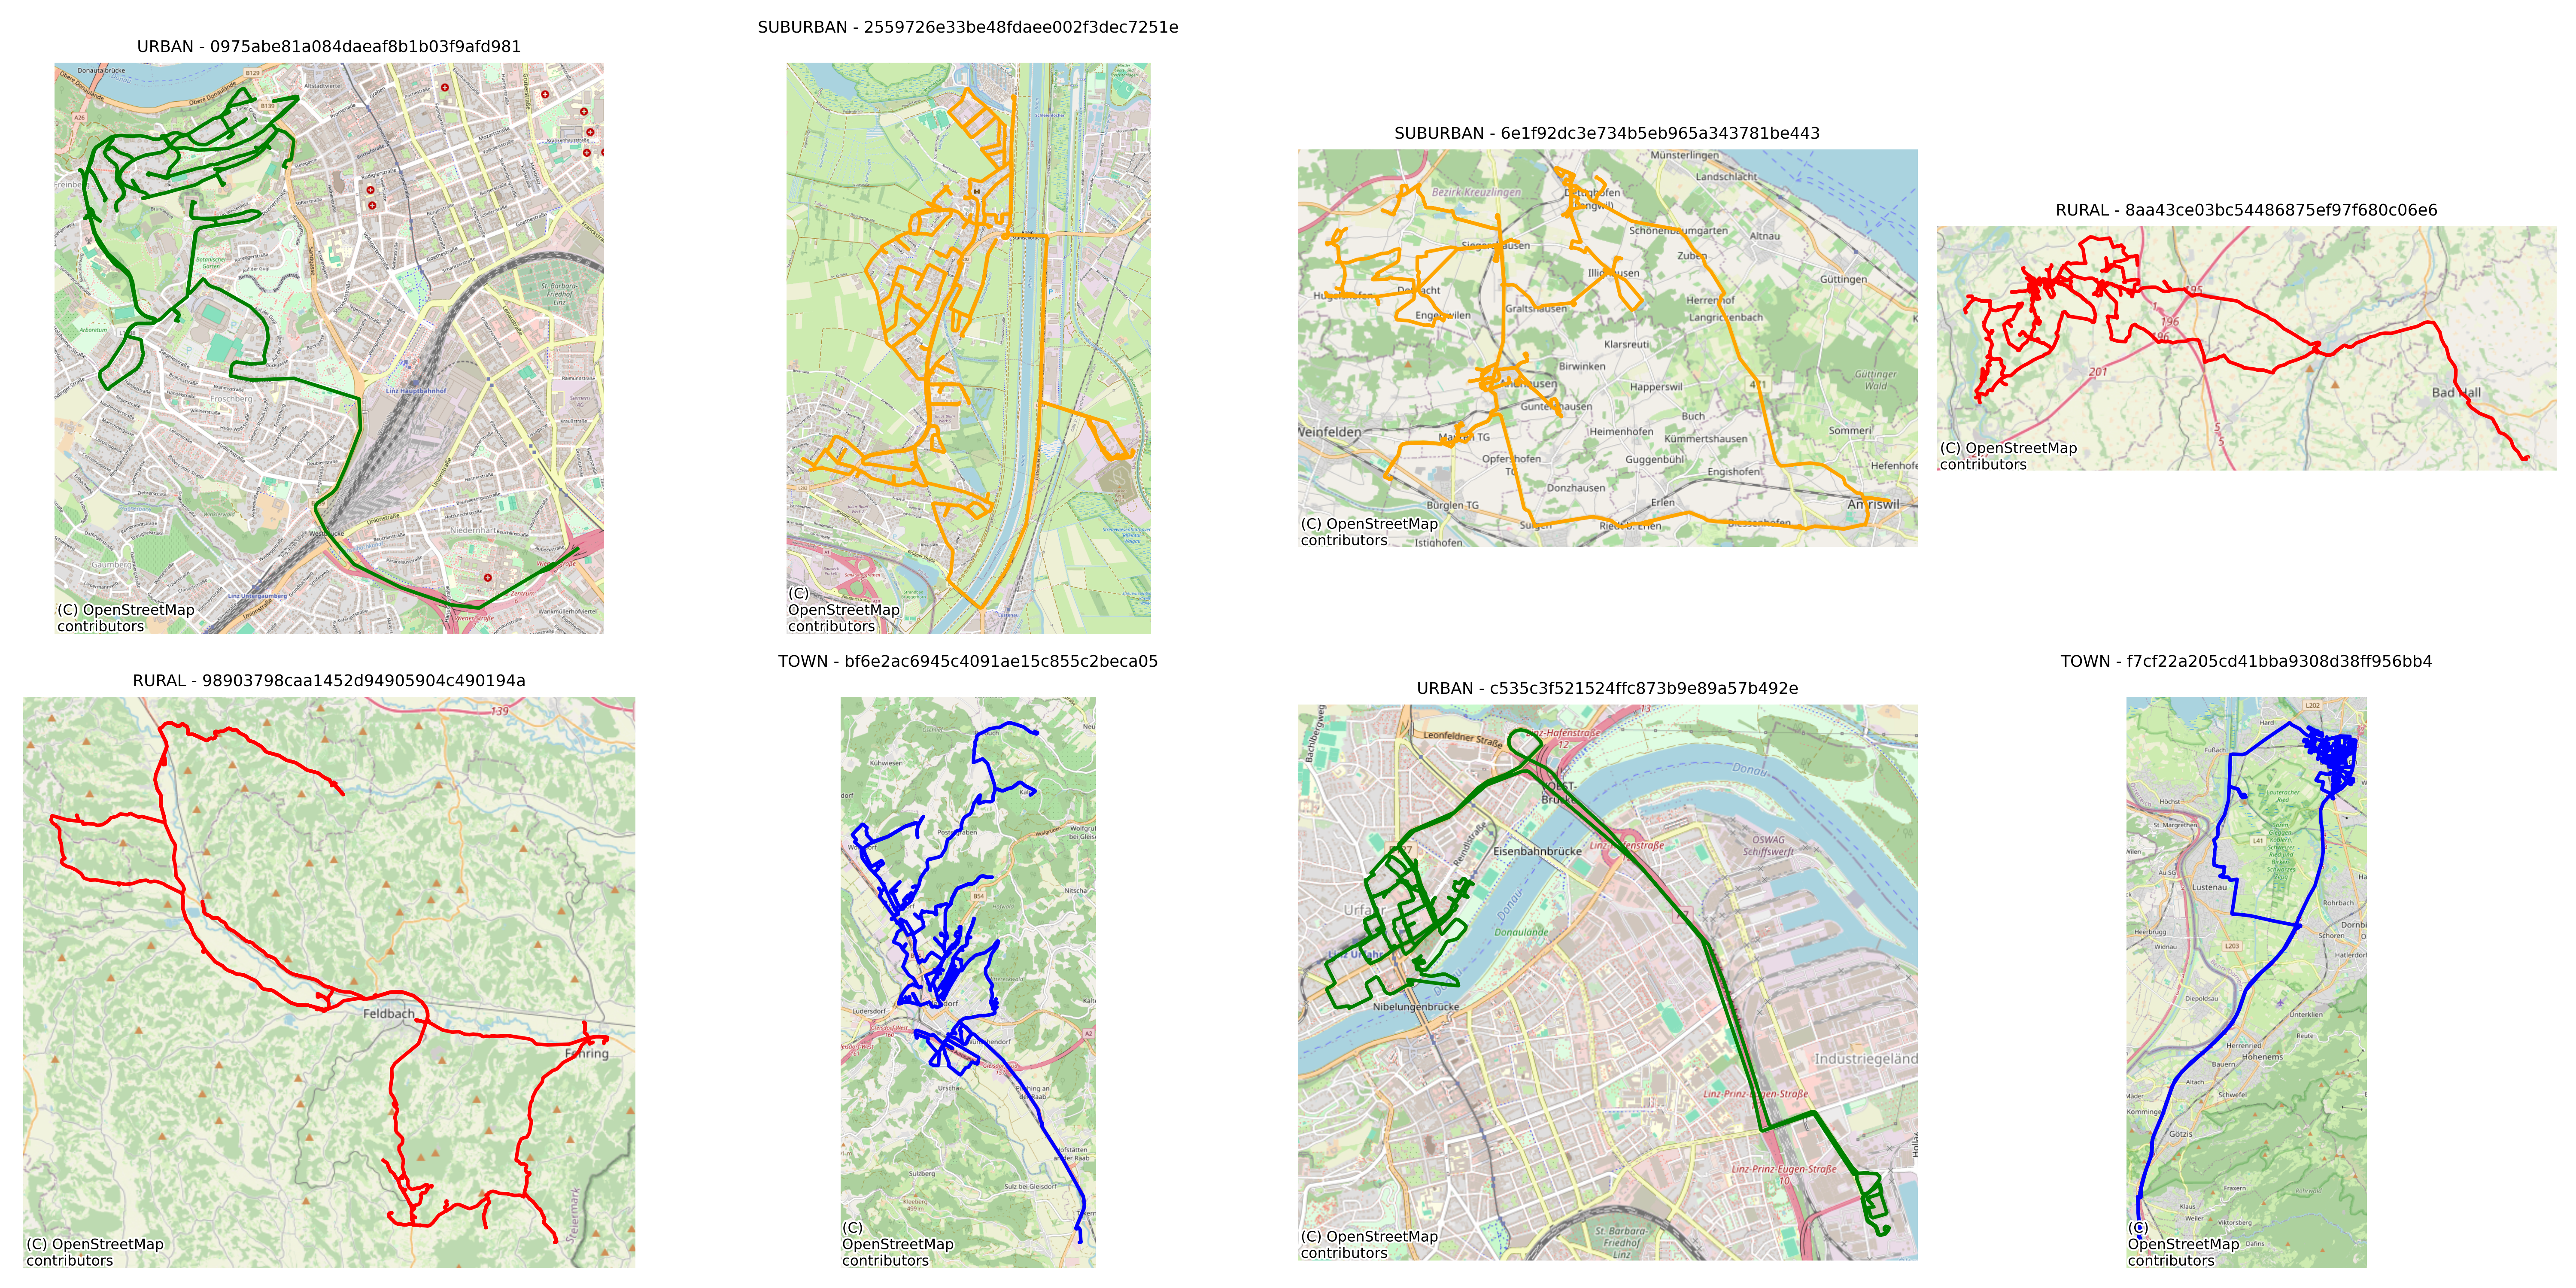
\includegraphics[width=\textwidth]{Figures/sample_tracking_routes_mapgrid.png}
  \caption{Mapgrid for selected sample trackings}
  \label{fig:sample_mapgrid}
\end{figure}
\FloatBarrier
The mapgrid shows spatial layout of each tracking route overlayed on a visual
map. Each subplot corresponds to a single tracking and is colorcoded with the
assigned lable (RURAL=Red, SUBURBAN=Orange, TOWN=Blue, URBAN=Green). This
visual representation clearly shows the difference in route shapes and sizes
between the four different area types.

\textbf{Urban:}
\begin{itemize}
  \item Routes are geographically compact and highly localized.
  \item Movement appears dense with short travel distances between stops.
  \item Often confined to a small cluster of city blocks or neighborhoods.
\end{itemize}

\textbf{Town:}
\begin{itemize}
  \item Coverage is slightly more dispersed than urban routes.
  \item Still relatively compact but less tightly packed.
  \item Serves a central area and nearby residential surroundings.
\end{itemize}

\textbf{Suburban:}
\begin{itemize}
  \item Routes extend farther and cover wider areas than town routes.
  \item Show transitional behavior between urban and rural structures.
  \item Less dense stop distribution, indicating more spaced-out residential
        zones.
\end{itemize}

\textbf{Rural:}
\begin{itemize}
  \item Routes are long and span large geographical areas.
  \item Stops are widely spaced, often connecting small, isolated settlements.
  \item The shape and path vary significantly, often following main roads
        between distant collection points.
\end{itemize}

\begin{figure}[htbp]
  \centering
  \includegraphics[width=\textwidth]{Figures/sample_pairplot.png}
  \caption{Pairplot of selected GPS route features grouped by area label}
  \label{fig:sample_pairplot}
\end{figure}
\FloatBarrier

The pairplot compares the relationships between the extracted features (eg.,
length, duration, number of points, bounding box area, point density, average
segmengt distance and number of stops). Rural and urban trackings show a clear
difference in multiple features. Point density and average segment distance are
especially good discriminators. Suburban and town trackings show more variance
and occasionally overlap with eachother, giving a not so clear distinction.

\begin{figure}[htbp]
  \centering
  \includegraphics[width=\textwidth]{Figures/sample_correlation_matrix.png}
  \caption{Correlation Matrix of selected GPS route features grouped by area
    label}
  \label{fig:sample_correlation_matrix}
\end{figure}
\FloatBarrier

The Correlation Matrix highlights the strong correlations between features in
the selected sample.
A high posive correlation between length, duration and number of points can be
observerd. Additionally the point density has a strong negative correlation
with the tracking length, number of points and average segment distance.

This correlation is to be expected and confirms the consistency of the data,
since the points (GPS coordinates) are recorded in uniform intervals. This plot
also indicates the possible redundance of features such as number of points and
number of stops.

\begin{figure}[h]
  \centering

  \includegraphics[width=\textwidth]{Figures/sample_point_density_boxplot.png}
  \caption{Boxplot of point density grouped by area label}
  \label{fig:sample_boxplot}
\end{figure}
\FloatBarrier

The point density boxplots for each label shows a clear difference between the
labels. Urban trackings appear to have the highest density and rural trackings
the lowest, with suburban and town trackings falling in the middle with a wider
variability.

This validates that the point density is a strong feature for classifying
trackings to the four labels.

\section{Solution Approach}
This chapter outlines the methods used to analyse and claaify the GPS tracking
data collected by waste collection vehicles.
The approach is structured in multiple stages, beginning with exploratory data
analysis, proceeding with feature extraction, data cleaning, outlier detection,
clustering and finally training a classifier.
The goal is to identify tracking patterns that allow for structural
classification of trackings into four categories: Urban, Suburban, Town and
Rural.

\subsection{Exploratory Data Analysis}

The foundation of this thesis is the dataset provided by \textit{infeo GmbH}.
It contains anonymized GPS track data collected by waste collection vehicles
during real world operation. Due to its large size of more than 100.000 GPS
tracks and its anonymization, a clear picture of the data needed to be
established as the first step.
With visual examination of different random trackings a sample of eight
manually labeled trackings was gathered.
The selected trackings were labeled to four categories, two trackings per
category.

\begin{itemize}
  \item Urban (Dense building structures, complex road networks, and minimal
        spacing between stops)
  \item Suburban (Moderately spaced residential areas with organized street
        layouts)
  \item Town (Smaller clustered settlements with simpler road structures)
  \item Rural (Sparse housing, long roads, large distances between collection
        points)
\end{itemize}

With the manually selected trackings varying in geographical structure, a
exploratory data
analysis helped transfer the visual distinction to clear differences found in
the data of each tracking category.

\subsection{Feature Extraction from Sample Dataset}
To enable the use of machine learning algorithms, each tracking originally
represented by a consecutive list of GPS waypoints with latitude and longitude
must be transformed into feature vectors. Feature extraction methods were
applied to derive representative metrics for each tracking.

This approach is well established and used in similar studies such as the
classification
of transportation modes by Etemad et al.~\cite{etemad_predicting_2018} and
clustering of GPS data using distance-based features by Koh et
al.~\cite{koh_clustering_2022}

\subsubsection{Features Available in Trackings}

\begin{enumerate}
  \item \textbf{Length:} Total distance of the route, in kilometers.
  \item \textbf{Duration:} Total time spent for the trackings, captured.
\end{enumerate}

\subsubsection{Features Extracted from Waypoints}

\begin{enumerate}
  \item \textbf{Number of Points:} The total number of GPS waypoints recorded
        in the tracking.
  \item \textbf{Bounding Box Area:} The area of the minimum bounding box that
        encloses all latitude and longitude waypoints in one tracking.
  \item \textbf{Point density:} The number of waypoints divided by the bounding
        box area. This feature indicates how closes packed the points are.
  \item \textbf{Average segment distance:} The mean distance between
        consecutive waypoints, computed using geodisc distance.
  \item \textbf{Number of Stops:} Waypoints with speed of zero. Originally
        considered as a potential feature, it was found out to be redundant as
        most
        waypoints have a speed of zero.
\end{enumerate}

\subsection{Filtering and Preprocessing the Full Dataset}
There are a lot of faulty datapoints that are not relevant for the
clustering, that are filtered out. Before applying machine learning methods,
extensive filtering was required to
remove invalid and irrelevant data from the dataset. These included:

\begin{enumerate}
  \item Trackings with a too low duration to be realistic collection trackings.

  \item Trackings that recorded movement only in and around a parking lot.
  \item Trackings left running overnight with no significant movement.
  \item Trackings with unrealistic GPS jumps and anomalies (possibly due to
        device errors or compression errors introduced by \textit{infeo GmbH}).
\end{enumerate}

Removing these faulty datapoints was curcial for ensuring the quality of the
clustering and reducing the computation times.

\subsection{Clustering and Pattern Discovery}
To discover patterns in the unlabeled dataset, clustering algorithhms were
applied.
Initially, K-Means++ was used to cluster the data into four clusters. However
the result showed that one cluster mostly consisted of outlier routes, with
unrealistic GPS jumps.

To solve this issue, the process was improved by detecting and removing
outliers using DBSCAN (Density-Based Spatial Clustering for Applications with
Noise). DBSCAN effectively removed most anomalies in the dataset. After
filtering the outliers with DBSCAN, K-Means++ clustering was applied again,
resulting clusters that represented the four defined categories better.

\subsection{Training a Classification Model}
% TODO: need to write more in this section
To automatically classify new trackings into one of the four categories (Urban,
Suburban, Town, Rural), a supervised machine learning model was trained using
the labeled dataset from the clustering step.

The labeled dataset was split into training and test sets using an 80/20 split.
Evaluation of the classifier on the test sset showed a high overall accuracy.

The trained classifier was saved for the later use in a sandbox API to classify
new trackings.

% TODO: Determine if the following three sections should be in the thesis or not
\subsection{Comparison with OSM Geofences}

\subsection{API Integration}

\section{Structure of the Work}

The remainder of this thesis is structured in the following chapters:

\begin{itemize}
  \item \textbf{Chapter 4: Implementation:} Provides a detailed description of
        how the previously introduced methos and algorithms were implemented.
        This
        includes the data preprocessing, feature extraction, clustering
        pipeline and
        classifier training.
  \item \textbf{Chapter 5: Evaluation and Discussion:} Presents the results of
        the clustering and classification. Performance metrics, visualizations,
        and
        analysis of the results are discussed alongside future reasearch and
        application.
  \item \textbf{Chapter 6: Conclusion:} Summarization of the contributions of
        the thesis, highlighting key takeaways and shortcomings.
\end{itemize}

This structure follows the development of the project, from understanding the
problem and analysing the data, to buildinng and evaluating a solution to
address the objective of classifying GPS trackings into structural categories.
\chapter{Implementation}

\section{Implementation of the Big Picture}

% oal: Translate the conceptual steps (from the big picture diagram) into real
% implementation stages.

% Bullet Points:

% Refer back to the high-level diagram from Chapter 3.

% Describe how each step (preprocessing, feature extraction, clustering,
% classification) is implemented in code (Python).

% Mention tools/libraries used: pandas, scikit-learn, geopy, DBSCAN, etc.

% Include a graphic: re-use or simplify the big-picture pipeline (could annotate
% it with function/module names).

% Optionally show a small code snippet or function signature for each step.

\begin{figure}[htbp]
  \centering

  \includegraphics[width=\textwidth]{Diagrams/drawio/big_picture_implementation.png}
  \caption{Big picture implementation pipeline}
  \label{fig:big_picture_implemetation_diagram}
\end{figure}
\FloatBarrier

\section{Data Handling and Preprocessing}
Preprocessing is a crucial step in the machine learning pipeline.

Each row in the dataset is a single GPS waypoint and consist of the following
columns:

\begin{itemize}
  \item \textbf{id\_tracking:} Unique identifier for each tracking.
  \item \textbf{sequence:} The order of the waypoint in the tracking.
  \item \textbf{latitude/longitude:} GPS coordinates.
  \item \textbf{speed:} Vehicle speed at the waypoint.
  \item \textbf{tracking\_duration:} Total time of the tracking.
  \item \textbf{tracking\_length:} Total dinstance of the tracking in km.
\end{itemize}

\subsection{Loading and Structuring the Dataset}

\subsection{Filtering Faulty Trackings}
The raw data included many invalid or irrelevant trackings that could impact
the analysis and clustering. These trackings were removed based on these
criteria:

\begin{itemize}
  \item \textbf{Duration Filter:} Trackings shorter than 30 minutes or longer
        than 10 hours were excluded.
  \item \textbf{Length Filter:} Trackings with a total length lower than 50 km
        or above 850km were excluded.
  \item \textbf{Minimal Waypoint Count:} Trackings with less than 10 recorded
        waypoints were excluded.
  \item \textbf{Minimal Bounding Box:} Trackings with a bounding box smaller
        than about 50 meters in latitude or longitude were excluded. This was a
        helpful
        step to reduce the amount of trackings that were exclusively recorded
        in a
        parking lot.
\end{itemize}

The filters were directly implemented as a SQL query executed in an jupyter
notebook. This reduced the further computatinal times for clustering and
training the classifier model. The SQL query implementing these filters looked
as follows:
\begin{lstlisting}[style=sql,caption={SQL query used for filtering the GPS tracking dataset},label={lst:sql-filter}]
  SELECT 
      wp.id_tracking, wp.id, wp.time, wp.type, wp.sequence, wp.comment, 
      wp.speed, wp.heading, wp.duration, wp.block_type, wp.log, 
      wp.latitude, wp.longitude, wp.altitude, wp.meta_tag, wp.meta_value,
      t.length AS tracking_length, 
      t.duration AS tracking_duration
  FROM waypoint wp
  JOIN tracking t ON wp.id_tracking = t.id
  WHERE 
      t.duration BETWEEN 18000000000 AND 360000000000  
      -- 0.5 to 10 hours
      AND t.length BETWEEN 50 AND 850  -- 50 to 850 km
      AND EXISTS (
          SELECT 1 FROM waypoint w 
          WHERE w.id_tracking = t.id
          HAVING COUNT(*) > 10  -- Min. 10 waypoints
      )
      AND (
          (SELECT MAX(latitude) FROM waypoint WHERE id_tracking = t.id) - 
          (SELECT MIN(latitude) FROM waypoint WHERE id_tracking = t.id)
      ) > 0.0005  -- Min. ~50m latitude span
      AND (
          (SELECT MAX(longitude) FROM waypoint WHERE id_tracking = t.id) - 
          (SELECT MIN(longitude) FROM waypoint WHERE id_tracking = t.id)
      ) > 0.0005;  -- Min. ~50m longitude span
  \end{lstlisting}

Each Filter step reduces the dataset by this many trackings:
\begin{table}[ht]
  \centering
  \begin{tabular}{|l|r|r|r|}
    \hline
    \textbf{Filter Step}     & \textbf{Remaining Trackings} &
    \textbf{Removed}
                             &
    \textbf{Reduction (\%)}
    \\
    \hline
    All trackings            & 101353                       & --
                             & --
    \\
    Duration filter          & 66477                        &
    34876
                             &
    34.410\%
    \\
    Length filter            & 45668                        &
    20809
                             &
    31.303\%
    \\
    Minimal Waypoints filter & 45599                        &
    69
                             &
    0.151\%
    \\
    Min Lat/Long span filter & 45598                        &
    1
                             &
    0.002\%
    \\
    \hline
    \textbf{Total Remaining} & \textbf{45598}               &
    \textbf{55755}
                             &
    \textbf{55.011\%}
    \\
    \hline
  \end{tabular}
  \caption{Tracking reduction per filtering step}
  \label{tab:filtering_summary}
\end{table}
\FloatBarrier

\section{Feature Extraction}

\subsection{Available Metadata Features}

\textbf{Tracking length}
\textbf{Tracking duration}

\subsection{Computed Features from Waypoints}

\paragraph{Number of points}

The total number of valid GPS points $n_p$ for a given route:
\[
  n_p = |\{(lat_i, lon_i)\}|
\]

\paragraph{Bounding box area}

The bounding box area $A_{bbox}$ is calculated as:
\[
  A_{bbox} = (\max(lat_i) - \min(lat_i)) \cdot (\max(lon_i) - \min(lon_i))
\]
This gives an approximation of the route’s spatial extent. A similar measure is
used in \cite{yang2009spatial} for comparing track spread.

\paragraph{Point density}

To measure how dense the GPS sampling is in space, we define point density
$d_p$ as:
\[
  d_p = \frac{n_p}{A_{bbox} + \varepsilon}
\]
where $\varepsilon$ is a small constant to avoid division by zero.

\paragraph{Average segment distance}

The average distance between consecutive waypoints $d_{avg}$:
\[
  d_{avg} = \frac{1}{n_p - 1} \sum_{i=1}^{n_p - 1} dist(p_i, p_{i+1})
\]
where \textit{dist} refers to the geodesic distance between two GPS points (in
meters), calculated using the WGS84 ellipsoid model.

\paragraph{Number of stops}

A stop is defined as a waypoint where the recorded speed equals zero. The
number of such points $n_s$ is computed as:
\[
  n_s = |\{i \mid speed_i = 0\}|
\]

\subsection{Feature Storage and Output}

The extracted features were stored in a structured csv file, with one row per
tracking\_id and all corresponding features. This resulting dataset forms the
basis for all future analysis, clustering and classification applications in
the next steps of the pipeline.

\begin{table}[h]
  \centering
  \begin{tabular}{ll}
    \textbf{Feature}                & \textbf{Description}
    \\
    \texttt{num\_points}            & Total GPS waypoints in the track
    \\
    \texttt{bbox\_area}             & Area covered by the track’s bounding box
    \\
    \texttt{point\_density}         & Points per unit area
    \\
    \texttt{avg\_segment\_distance} & Mean distance between consecutive
    points
    \\
    \texttt{num\_stops}             & Count of zero-speed positions
    \\
    \texttt{duration}               & Duration of tracking (from metadata)
    \\
    \texttt{length}                 & Route length in meters (from metadata)
    \\
  \end{tabular}
  \caption{Overview of extracted features per tracking.}
\end{table}

\section{Clustering Implementation}

\begin{figure}[htbp]
  \centering

  \includegraphics[width=1\textwidth]{Figures/histogram_feature_data_pre_clustering.png}
  \caption{Histogram}
  \label{fig:histogram-feature-engineered-data}
\end{figure}
\FloatBarrier

\begin{figure}[htbp]
  \centering

  \includegraphics[width=1\textwidth]{Figures/correlation_matrix_pre_clustering.png}
  \caption{Correlation matrix}
  \label{fig:correlation-matrix}
\end{figure}
\FloatBarrier

\subsection{DBSCAN for Outlier Removal}

\begin{figure}[htbp]
  \centering

  \includegraphics[width=0.9\textwidth]{Figures/dbscan_diagram_feature_data.png}
  \caption{DBSCAN}
  \label{fig:dbscan-clustering-outlier-removal}
\end{figure}
\FloatBarrier

\subsection{K-Means for Category Discovery}

\begin{figure}[htbp]
  \centering

  \includegraphics[width=0.9\textwidth]{Figures/kmeans_diagram_feature_data.png}
  \caption{K-means clustering}
  \label{fig:kmeans-clustering}
\end{figure}
\FloatBarrier

\section{Classification Model}

\subsection{Model Selection and Training}

\subsection{Feature Importance Analysis}

\subsection{Saving and Exporting the Classifier}

\section{Integration with existing systems}
Formatvorlage für den Fließtext.

\chapter{Evaluation and Discussion}

\section{Definition of the data sets used for the evaluation}
Formatvorlage für den Fließtext.

\section{Evaluation of the results}
Formatvorlage für den Fließtext.

\begin{figure}[htbp]
  \centering

  \includegraphics[width=0.9\textwidth]{Figures/classifier/boxplots/classifier_bbox_area_boxplot.png}
  \caption{Bounding Box Boxplot}
  \label{fig:bbox_boxplot_classifier}
\end{figure}
\FloatBarrier
\begin{figure}[htbp]
  \centering

  \includegraphics[width=0.9\textwidth]{Figures/classifier/boxplots/classifier_point_density_boxplot.png}
  \caption{Point Density Boxplot}
  \label{fig:point_density_boxplot_classifier}
\end{figure}
\FloatBarrier

\begin{figure}[htbp]
  \centering

  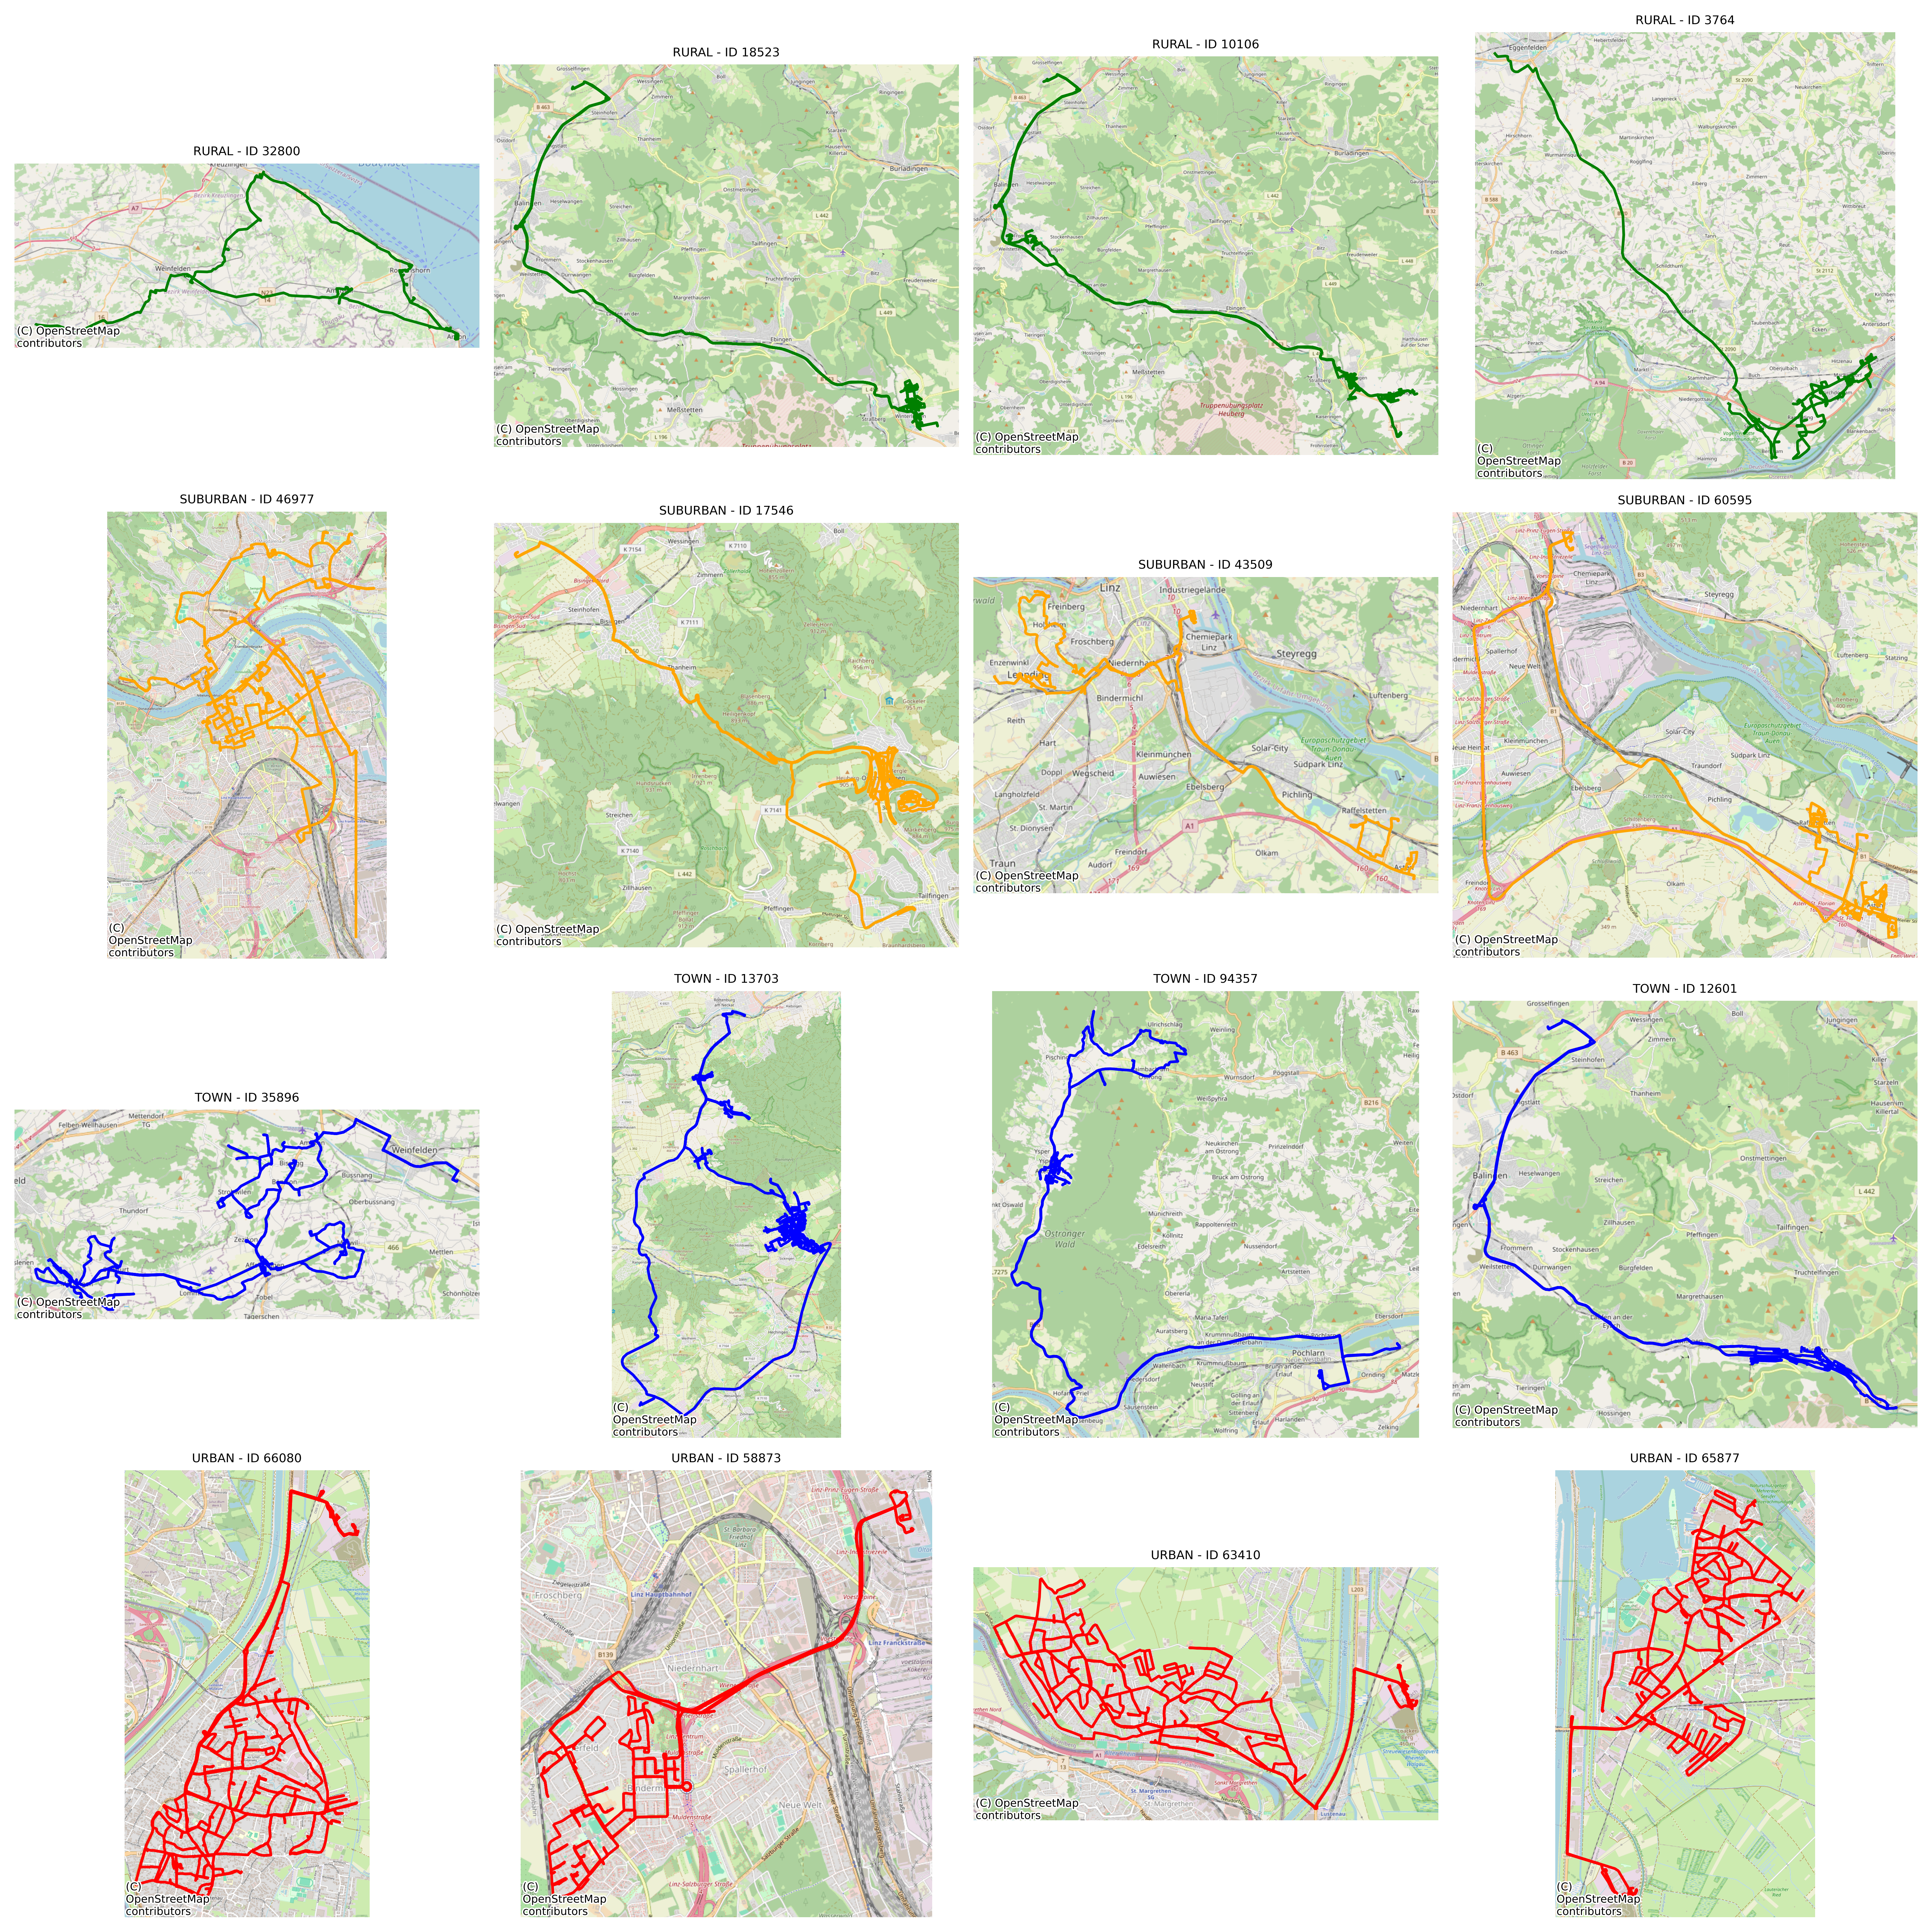
\includegraphics[width=\textwidth]{Figures/classifier/four_final_predictions_per_class.png}
  \caption{Randomforest classifier predictions on testset}
  \label{fig:four_final_predictions_on_testset}
\end{figure}
\FloatBarrier
\section{Reflection on the results}
Formatvorlage für den Fließtext.

\chapter{Conclusion}

\section{Future Directions}
Formatvorlage für den Fließtext.

\section{Limitations}
Formatvorlage für den Fließtext.

Literaturverzeichnis:
\clearpage
\phantomsection
\addcontentsline{toc}{chapter}{Literaturverzeichnis}
\printbibliography

% \chapter*{[evtl. Anhang]}  % evtl. ersetzen mit \chapter*{Anhang}
% \addcontentsline{toc}{chapter}{[evtl. Anhang]}
% % evtl. ersetzen mit \addcontentsline{toc}{chapter}{Anhang}
% Formatvorlage für den Fließtext.

% \section{Use of AI tools}

% \begin{table}[h]
%   \centering
%   \caption{Use of AI tools during the creation process}
%   \label{tab:ai_usage}
%   \resizebox{\textwidth}{!}{%
%     \begin{tabular}{|p{3.2cm}|c|c|p{5.5cm}|}
%       \hline
%       \textbf{Working step}                  & \textbf{AI used}
%                                              & \textbf{AI
%       tool(s)}                               &
%       \textbf{Experiences / recommendations / irritations}
%       \\
%       \hline
%       Find a topic idea                      & no
%                                              & -
%                                              & -
%       \\
%       \hline
%       Narrow down topic / Formulate question & no
%                                              & -
%                                              & -
%       \\
%       \hline
%       Find sources                           & yes
%                                              & OpenAI GPT-4o
%                                              & Helped identify relevant
%       keywords and
%       topic clusters.
%       \\
%       \hline
%       Explain terms                          & yes
%                                              & OpenAI GPT-4o
%                                              & Useful for quick definitions and
%       simple explanations.
%       \\
%       \hline
%       Design text structure                  & yes
%                                              & OpenAI GPT-4o
%                                              & Good for outlining sections.
%       Required manual adjustments.
%       \\
%       \hline
%       Have content read aloud                & no
%                                              & -
%                                              & -
%       \\
%       \hline
%       Translate content                      & no
%                                              & -
%                                              & -
%       \\
%       \hline
%       Dictate content                        & no
%                                              & -
%                                              & -
%       \\
%       \hline
%       Paraphrase content, summarise          & yes
%                                              & OpenAI GPT-4o
%                                              & Helpful to generate
%       concise summaries of long text.
%       \\
%       \hline
%       Write introduction                     & yes
%                                              & OpenAI GPT-4o
%                                              & Provided inspiration but
%       required rewording.
%       \\
%       \hline
%       Write main chapter                     & yes
%                                              & OpenAI GPT-4o
%                                              & Used for structuring and
%       rephrasing, not full writing.
%       \\
%       \hline
%       Write a summary                        & yes
%                                              & OpenAI GPT-4o
%                                              & Used to condense main points
%       effectively.
%       \\
%       \hline
%       Obtain text feedback                   & yes
%                                              & OpenAI GPT-4o
%                                              & Used to review tone, clarity,
%       and consistency.
%       \\
%       \hline
%       Revise text statement                  & yes
%                                              & OpenAI GPT-4o
%                                              & Helpful for reformulating
%       statements.
%       \\
%       \hline
%       Revise text formulation                & yes
%                                              & OpenAI GPT-4o
%                                              & Polished sentences and
%       improved flow.
%       \\
%       \hline
%       Correct text formally                  & yes
%                                              & OpenAI GPT-4o
%                                              & Assisted with grammar and
%       punctuation checking.
%       \\
%       \hline
%       Code generation                        & yes
%                                              & OpenAI GPT-4o, Github Copilot
%                                              & Assisted with generating code
%       and fixing bugs
%       \\
%       \hline
%     \end{tabular}%
%   }
% \end{table}

\chapter*{Affidavit}
\addcontentsline{toc}{chapter}{Affidavit}
I hereby declare in lieu of oath that I have written this Bachelor
thesis independently and without the use of aids other than those specified.
The passages taken directly or indirectly from other sources
directly or indirectly from other sources are marked as such. The thesis has
not been
neither in the same nor in a similar form to any other examination authority
nor has it been published.

\vspace{3cm}
\noindent
Dornbirn, on 15. May 2025\hfill Matthias Hefel

\end{document}
